% ----------------------------------------------------------
\chapter{Método de Hueckel} \label{ap:HMO}
% ----------------------------------------------------------

Considerando métodos semi-empíricos fundamentados na teoria \gls{HF}, pode-se citar o \gls{HMO}, no qual se aplicam as devidas aproximações resultantes dos conceitos e dados experimentais, pois estes tendem a ser intuitivos. Em alcenos e alcinos, os elétrons-$\pi$ estão presentes nos orbitais p, os quais são considerados como independentes da estrutura sigma dos orbitais híbridos e elétrons sigma. Funções de onda $\psi$ é dada pela \autoref{ap:eq:1}.

\begin{figure}[htb]
    \vspace{2\baselineskip}
\begin{equation}
    \label{ap:eq:1}
    \psi = \tikzmarknode{coefficient}{\highlight{red}{$a_1$}} \tikzmarknode{wavefunction}{\highlight{blue}{$\phi_1$}} + a_2\phi_2 + \dots + a_i \phi_i
\end{equation}
\begin{tikzpicture}[overlay,remember picture,>=stealth,nodes={align=left,inner ysep=1pt},<-]
    \path (wavefunction.north) ++ (-1.2em,1.5em) node[anchor=south east,color=blue!67] (scalep){\textit{função de onda}};
    \draw [color=blue!87](wavefunction.north) |- ([xshift=-3em,color=blue]scalep.south west);
    
    \path (coefficient.south) ++ (1.2em,-1.5em) node[anchor=north west,color=red!67] (scalep){\textit{coeficiente de contribuição}};
    \draw [color=red!87](coefficient.south) |- ([xshift=3em,color=red]scalep.north east);
\end{tikzpicture}
\end{figure}

Como somente os elétrons dos orbitais p estão contribuindo para a função de onda, a \autoref{ap:eq:1} pode ser escrita como a \autoref{ap:eq:2}.

\begin{figure}[htb]
    \vspace{2\baselineskip}
\begin{equation}
    \label{ap:eq:2}
    \psi = a_1 p_1 + a_2 p_2 + \dots + a_i p_i
\end{equation}
\end{figure}

Tomando o eteno como exemplo, pode-se afirmar que cada carbono contribui com um elétron para a ligação $\pi$, sendo $p_1$ e $p_2$ os elétrons dos átomos de carbono 1 e 2, cujas respectivas contribuições são ponderadas por $a_1$ e $a_2$. No caso dos orbitais p não hibridizados, os orbitais moleculares são formados pela \gls{LCAO} $p_1$ e $p_2$. Sobreposição entre orbitais atômicos podem ocorrer de forma simétrica (resultando em um orbital ligante) ou antissimétrica (formando um orbital antiligante).

\begin{figure}[htb]
    \vspace{2\baselineskip}
\begin{equation}
    \label{ap:eq:3}
    \psi =
    \begin{cases}
\tikzmarknode{simetric}{\highlight{blue}{$\psi^+$}} = a_1 p_1 + a_2 p_2 \\
\tikzmarknode{antissimetric}{\highlight{red}{$\psi^-$}} = a_1 p_1 - a_2 p_2
    \end{cases}
\end{equation}
\begin{tikzpicture}[overlay,remember picture,>=stealth,nodes={align=left,inner ysep=1pt},<-]
    \path (simetric.north) ++ (-1.2em,1.5em) node[anchor=south east,color=blue!67] (scalep){\textit{função simétrica}};
    \draw [color=blue!87](simetric.north) |- ([xshift=-3em,color=blue]scalep.south west);
    
    \path (antissimetric.south) ++ (1.2em,-1.5em) node[anchor=north west,color=red!67] (scalep){\textit{função antissimétrica}};
    \draw [color=red!87](antissimetric.south) |- ([xshift=3em,color=red]scalep.north east);
\end{tikzpicture}
\end{figure}

Usando a \autoref{ap:eq:4} (equação de Schroedinger) como base fundamental para avançar na discussão do cálculo dos valores de energia associados aos orbitais, pode-se aplicar o princípio variacional como uma aproximação necessária e conveniente para encontrar as funções de minimização da energia relativa aos orbitais no estado fundamental. Este método consiste em escolher uma função de onda inicial que dependa de um ou mais parâmetros, e encontrar os valores destes parâmetros para cada valor esperado onde a energia seja a menor possível. A função de onda obtida na substituição dos parâmetros pelos valores encontrados será uma aproximação do estado fundamental da função de onda, e o valor esperado de energia neste estado será majorante para a energia deste estado fundamental.

%%% TODO: explicar o princípio variacional 

\begin{figure}[htb]
    \vspace{2\baselineskip}
\begin{equation}
\label{ap:eq:4}
    \tikzmarknode{hamiltonian}{\highlight{red}{$\hat{H}$}} \psi = \tikzmarknode{energy}{\highlight{blue}{$E$}} \psi
\end{equation}
\begin{tikzpicture}[overlay,remember picture,>=stealth,nodes={align=left,inner ysep=1pt},<-]
    \path (energy.north) ++ (-1.2em,1.5em) node[anchor=south east,color=blue!67] (scalep){\textit{energia}};
    \draw [color=blue!87](energy.north) |- ([xshift=-3em,color=blue]scalep.south west);
    
    \path (hamiltonian.south) ++ (1.2em,-1.5em) node[anchor=north west,color=red!67] (scalep){\textit{operador}};
    \draw [color=red!87](hamiltonian.south) |- ([xshift=3em,color=blue]scalep.north east);
\end{tikzpicture}
\end{figure}

\begin{equation}
\label{ap:eq:5}
    \psi \hat{H} \psi = \psi^2 E
\end{equation}

Multiplicando ambos os lados por $\psi$, obtém-se a \autoref{ap:eq:5}. Aplicado a integral nessa expressão (mantendo a igualdade) e, em seguida, isolando a energia $E$, obtém-se a \autoref{ap:eq:6}.

\begin{equation}
\label{ap:eq:6}
    E = \frac{\displaystyle \int \psi \hat{H} \psi d\tau}{\displaystyle \int \psi^2 d\tau}
\end{equation}

Na \autoref{ap:eq:5}, a energia esperada vai ser superestimada em relação ao valor real. Desse modo, o resultado calculado vai ser minimizado através de um procedimento matemático submetido a um conjunto de funções de base. No caso do eteno (\ce{C_2 H_2}), podemos substituir o termo $\psi$ da \autoref{ap:eq:6} pela \autoref{ap:eq:2}, obtendo a \autoref{ap:eq:7}.

\begin{figure}[htb]
    \vspace{2\baselineskip}
\begin{equation}
\label{ap:eq:7}
    E = \frac{\displaystyle \int \tikzmarknode{LCAO}{\highlight{blue}{$(a_1 p_1 + a_2 p_2)$}} \hat{H} \highlight{blue}{$(a_1 p_1 + a_2 p_2)$} d\tau}{\displaystyle \int \highlight{blue}{$(a_1 p_1 + a_2 p_2)$}^2 d\tau}
\end{equation}
\begin{tikzpicture}[overlay,remember picture,>=stealth,nodes={align=left,inner ysep=1pt},<-]
    \path (LCAO.north) ++ (1.2em,1.5em) node[anchor=south west,color=blue!67] (scalep){LCAO \textit{do eteno}};
    \draw [color=blue!87](LCAO.north) |- ([xshift=3em,color=blue]scalep.south east);
\end{tikzpicture}
\end{figure}

Abrindo a expressão da \autoref{ap:eq:7}, é possível isolar as seguintes integrais:

\begin{figure}[htb]
    \vspace{2\baselineskip}
\begin{equation}
\label{ap:eq:8}
    \displaystyle \int (p_1 \hat{H} p_1) d\tau = \tikzmarknode{alpha}{\highlight{blue}{$\alpha$}} \\
\end{equation}
\begin{tikzpicture}[overlay,remember picture,>=stealth,nodes={align=left,inner ysep=1pt},<-]
    \path (alpha.north) ++ (-1.2em,1.5em) node[anchor=south east,color=blue!67] (scalep){\textit{integral de Coulomb}};
    \draw [color=blue!87](alpha.north) |- ([xshift=-3em,color=blue]scalep.south west);
\end{tikzpicture}
\end{figure}

A integral de Coulomb, mostrada na \autoref{ap:eq:8}, é o Hamiltoniano para a energia de Coulomb relativa a um elétron com uma função de onda $p_i$ no campo do átomo $i$ e influenciado pelo seu núcleo. Esse elétron não sofre efeito de nenhum outro núcleo. Essa aproximação funciona melhor quando os átomos das vizinhanças não possuem cargas elétricas. Ou seja, $\alpha$ é uma função da carga nuclear e do tipo de orbital. Por ser um termo atrativo, possui um valor negativo. 

\begin{figure}[htb]
    \vspace{2\baselineskip}
\begin{equation}
\label{ap:eq:9}
    \displaystyle \int (p_1 \hat{H} p_2) d\tau = \displaystyle \int (p_2 \hat{H} p_1) d\tau = \tikzmarknode{beta}{\highlight{blue}{$\beta$}}
\end{equation}
\begin{tikzpicture}[overlay,remember picture,>=stealth,nodes={align=left,inner ysep=1pt},<-]
    \path (beta.north) ++ (-1.2em,1.5em) node[anchor=south east,color=blue!67] (scalep){\textit{integral de troca (ou de \textbf{ressonância})}};
    \draw [color=blue!87](beta.north) |- ([xshift=-3em,color=blue]scalep.south west);
\end{tikzpicture}
\end{figure}

As integrais de sobreposição são dadas pelas expressões na \autoref{ap:eq:10}. Se $i=j$, então $S_{ii} = \displaystyle \int p_i p_i d \tau$ para os orbitais atômicos normalizados. Se $i \neq j $, a integral de sobreposição é igual a $0$ para os orbitais atômicos ortogonais. Ou seja, o valor de $S$ varia de $0$ a $1$ e representa uma medida da não-ortogonalidade dos orbitais. Uma vez que as funções $p$ dos orbitais são amplamente separadas no espaço e são independentes, espera-se que elas sejam ortogonais.

\begin{figure}[htb]
    \vspace{2\baselineskip}
\begin{equation}
\label{ap:eq:10}
\displaystyle \int (p_i p_j) d\tau =
\begin{cases}
 \tikzmarknode{s11}{\highlight{blue}{$S_{11}$}} = \displaystyle \int (p_1 p_1) d\tau = \highlight{blue}{$S_{22}$} = \displaystyle \int (p_2 p_2) d\tau \\
 \tikzmarknode{s12}{\highlight{red}{$S_{12}$}} = \displaystyle \int (p_2 p_1) d\tau = \highlight{red}{$S_{21}$} = \displaystyle \int (p_1 p_2) d\tau
\end{cases}
\end{equation}
\begin{tikzpicture}[overlay,remember picture,>=stealth,nodes={align=left,inner ysep=1pt},<-]
    \path (s11.north) ++ (1.2em,1.5em) node[anchor=south west,color=blue!67] (scalep){\textit{integral de sobreposição ($i = j$)}};
    \draw [color=blue!87](s11.north) |- ([xshift=3em,color=blue]scalep.south east);
    
    \path (s12.south) ++ (1.2em,-1.5em) node[anchor=north west,color=red!67] (scalep){\textit{integral de sobreposição ($i \neq j$)}};
    \draw [color=red!87](s12.south) |- ([xshift=3em,color=red]scalep.north east);
\end{tikzpicture}
\end{figure}

Com as simplificações feitas anteriormente, é possível reescrever a expressão que calcula a energia para a molécula de eteno de acordo com a \autoref{ap:eq:12}.

\begin{figure}[htb]
    \vspace{2\baselineskip}
\begin{equation}
\label{ap:eq:12}
    E = \frac{\tikzmarknode{numerador}{\highlight{blue}{$a_1^2 \alpha + 2a_1 a_2 \beta + a_2^2 \alpha$}}}{\tikzmarknode{denominador}{\highlight{red}{$a_1^2 S_{11} + 2a_1 a_2 S_{12} + a_2^2 S_{22}$}}}
\end{equation}
\begin{tikzpicture}[overlay,remember picture,>=stealth,nodes={align=left,inner ysep=1pt},<-]
    \path (numerador.north) ++ (1.2em,1.5em) node[anchor=south west,color=blue!67] (scalep){\textit{numerador($N$)}};
    \draw [color=blue!87](numerador.north) |- ([xshift=3em,color=blue]scalep.south east);
    
    \path (denominador.south) ++ (1.2em,-1.5em) node[anchor=north west,color=red!67] (scalep){\textit{denominador($D$)}};
    \draw [color=red!87](denominador.south) |- ([xshift=3em,color=red]scalep.north east);
\end{tikzpicture}
\end{figure}

Desse modo, conhecendo $\alpha$, $\beta$ e $S$, a energia pode ser calculada. O critério de minimização em relação a alguns parâmetros é mostrado na \autoref{ap:eq:12}.

\begin{figure}[htb]
    \vspace{2\baselineskip}
\begin{equation}
\label{ap:eq:13}
    \frac{\partial E}{\partial a_1} = \frac{\partial E}{\partial a_2} = 0
\end{equation}
\end{figure}

Como alternativa, ao invés de variar a função teste para encontrar o valor mínimo de $E$ (\autoref{ap:eq:12}), pode-se variar os coeficientes lineares. Esse é um caso direto da busca pelo mínimo de uma função. Aplicando, então, a condição da \autoref{ap:eq:13}, obtém-se a \autoref{ap:eq:13a}.

\begin{figure}[htb]
    \vspace{2\baselineskip}

\begin{align}
\label{ap:eq:13a}
   \frac{\partial E}{\partial a_1} = \frac{\tikzmarknode{nlinha}{\highlight{blue}{$N'$}}D - E \tikzmarknode{dlinha}{\highlight{red}{$D'$}}}{D^2} = \frac{N' - ED'}{D} = 0 \\[0.3cm]
    \frac{\partial E}{\partial a_2} = \frac{\tikzmarknode{nlinha2}{\highlight{blue}{$N'$}}D - E \tikzmarknode{dlinha2}{\highlight{red}{$D'$}}}{D^2} = \frac{N' - ED'}{D} = 0
\end{align}
\begin{tikzpicture}[overlay,remember picture,>=stealth,nodes={align=left,inner ysep=1pt},<-]
    \path (nlinha.north) ++ (-1.2em,1.5em) node[anchor=south east,color=blue!67] (scalep){\textit{$2(a_1 \alpha + a_2 \beta)$}};
    \draw [color=blue!87](nlinha.north) |- ([xshift=-3em,color=blue]scalep.south west);
    
    \path (dlinha.north) ++ (1.2em,1.5em) node[anchor=south west,color=red!67] (scalep){\textit{$2(a_1 S_{11} + a_2 S_{12})$}};
    \draw [color=red!87](dlinha.north) |- ([xshift=3em,color=red]scalep.south east);
    
    \path (nlinha2.south) ++ (-1.5em,-1.8em) node[anchor=north east,color=blue!67] (scalep){\textit{$2(a_1 \beta + a_2 \alpha)$}};
    \draw [color=blue!87](nlinha2.south) |- ([xshift=-3em,color=blue]scalep.north west);
    
    \path (dlinha2.south) ++ (1.5em,-1.8em) node[anchor=north west,color=red!67] (scalep){\textit{$2(a_1 S_{11} + a_2 S_{12})$}};
    \draw [color=red!87](dlinha2.south) |- ([xshift=3em,color=red]scalep.north east);
\end{tikzpicture}
\end{figure}

Simplificando \autoref{ap:eq:13a}, temos que $N' - ED' = 0$ e, portanto, $N' = ED'$. Desse modo, fazendo as substituições obtidas nas expressões da  \label{ap:eq:13a}, obtemos a \autoref{ap:eq:13b}.

\begin{figure}[htb]
    \vspace{2\baselineskip}
\begin{align}
\label{ap:eq:13b}
    a_1 \alpha + a_2 \beta = E(a_1 S_{11} + a_2 S_{12}) \\[0.35cm]
    a_1 \beta - E a_1 S_{12} + a_2 \alpha - E a_2 S_{22} = 0 \\[0.35cm]
    a_1 (\beta - ES_{12}) + a_2 (\alpha - ES_{22}) = 0
\end{align}
\end{figure}

Para prosseguir, assumimos que as funções de onda $p_1$ e $p_2$ retêm a condição de ortonormalidade, mesmo no estadop molecular. Ou seja, $S_{12} = S_{21} = 0$ e $S_{11} = S_{22} = 1$. Substituindo essas aproximações nas equações anteriores, temos:

\begin{figure}[htb]
    \vspace{2\baselineskip}
\begin{align}
\label{ap:eq:13b}
    a_1 (\alpha - E) + a_2 \beta = 0 \\[0.35cm]
    a_2 (\alpha - E) + a_1 \beta = 0
\end{align}
\end{figure}

Essas equações ortonormais são chamadas equações seculares, cujos coeficientes podem ser transformados em uma matriz quadrada, para o caso do eteno (\autoref{ap:eq:13c}). A partir dessa matriz, a solução de $E$ é computacionalmente simples, uma vez que este é autovalor da matriz secular dos coeficientes.

\begin{equation}
\label{ap:eq:13c}
\begin{bmatrix}
    (\alpha - E) & \beta \\
    \beta  & (\alpha - E)
\end{bmatrix}
\end{equation}

Se dividirmos os elementos da matriz representada na \autoref{ap:eq:13c} por $\beta$, obtemos a \autoref{ap:eq:13d}, que pode ainda ser reduzida à \autoref{ap:eq:13e}.

\begin{figure}[htb]
    \vspace{3 \baselineskip}
\begin{equation}
\label{ap:eq:13d}
\begin{bmatrix}
    \displaystyle \tikzmarknode{term}{\highlight{blue}{$ \displaystyle \frac{(\alpha - E)}{\beta}$}} & 1 \\
    1  & \highlight{blue}{$\displaystyle \frac{(\alpha - E)}{\beta}$}
\end{bmatrix}
\end{equation}
\begin{tikzpicture}[overlay,remember picture,>=stealth,nodes={align=left,inner ysep=1pt},<-]
    \path (term.north) ++ (1.2em,1.5em) node[anchor=south west,color=blue!67] (scalep){\textit{$\displaystyle x = \frac{(\alpha - E)}{\beta}$}};
    \draw [color=blue!87](term.north) |- ([xshift=3em,color=blue]scalep.south east);
\end{tikzpicture}
\end{figure}

\begin{equation}
\label{ap:eq:13e}
\begin{bmatrix}
    x & 1 \\
    1  & x
\end{bmatrix}
\end{equation}

A solução dessa matriz (\autoref{ap:eq:13e}) pode ser obtida simplesmente pela expansão do determinante correspondente (determinante secular) ou encontrando os autovalores e autovetores da matriz (matriz secular). Como a situação envolve dependência linear, o determinante secular deve ser igual a zero.

\begin{equation}
    \begin{vmatrix}
    x & 1 \\
    1  & x
\end{vmatrix}
= 0 \implies
\begin{cases}
 x^2 - 1 = 0 \\
 x^2 = 1 \\
 x = \pm 1
\end{cases}
\end{equation}

Assim, para o eteno, nós obtemos dois autovalores: $E = \alpha - \beta$ e $E = \alpha + \beta$, gerando um diagrama de orbitais moleculares \autoref{fig:A2}. Essa metodologia pode ser generalizada por sistemas conjugados de qualquer tamanho. Desse modo, dimensão da matriz na \autoref{ap:eq:13c} é dada pelo número de átomos no sistema $\pi$ conjugado.

\begin{figure}[htb]
	\caption{\label{fig:A2} Orbitais moleculares de Hueckel para o eteno.}
	\begin{center}
		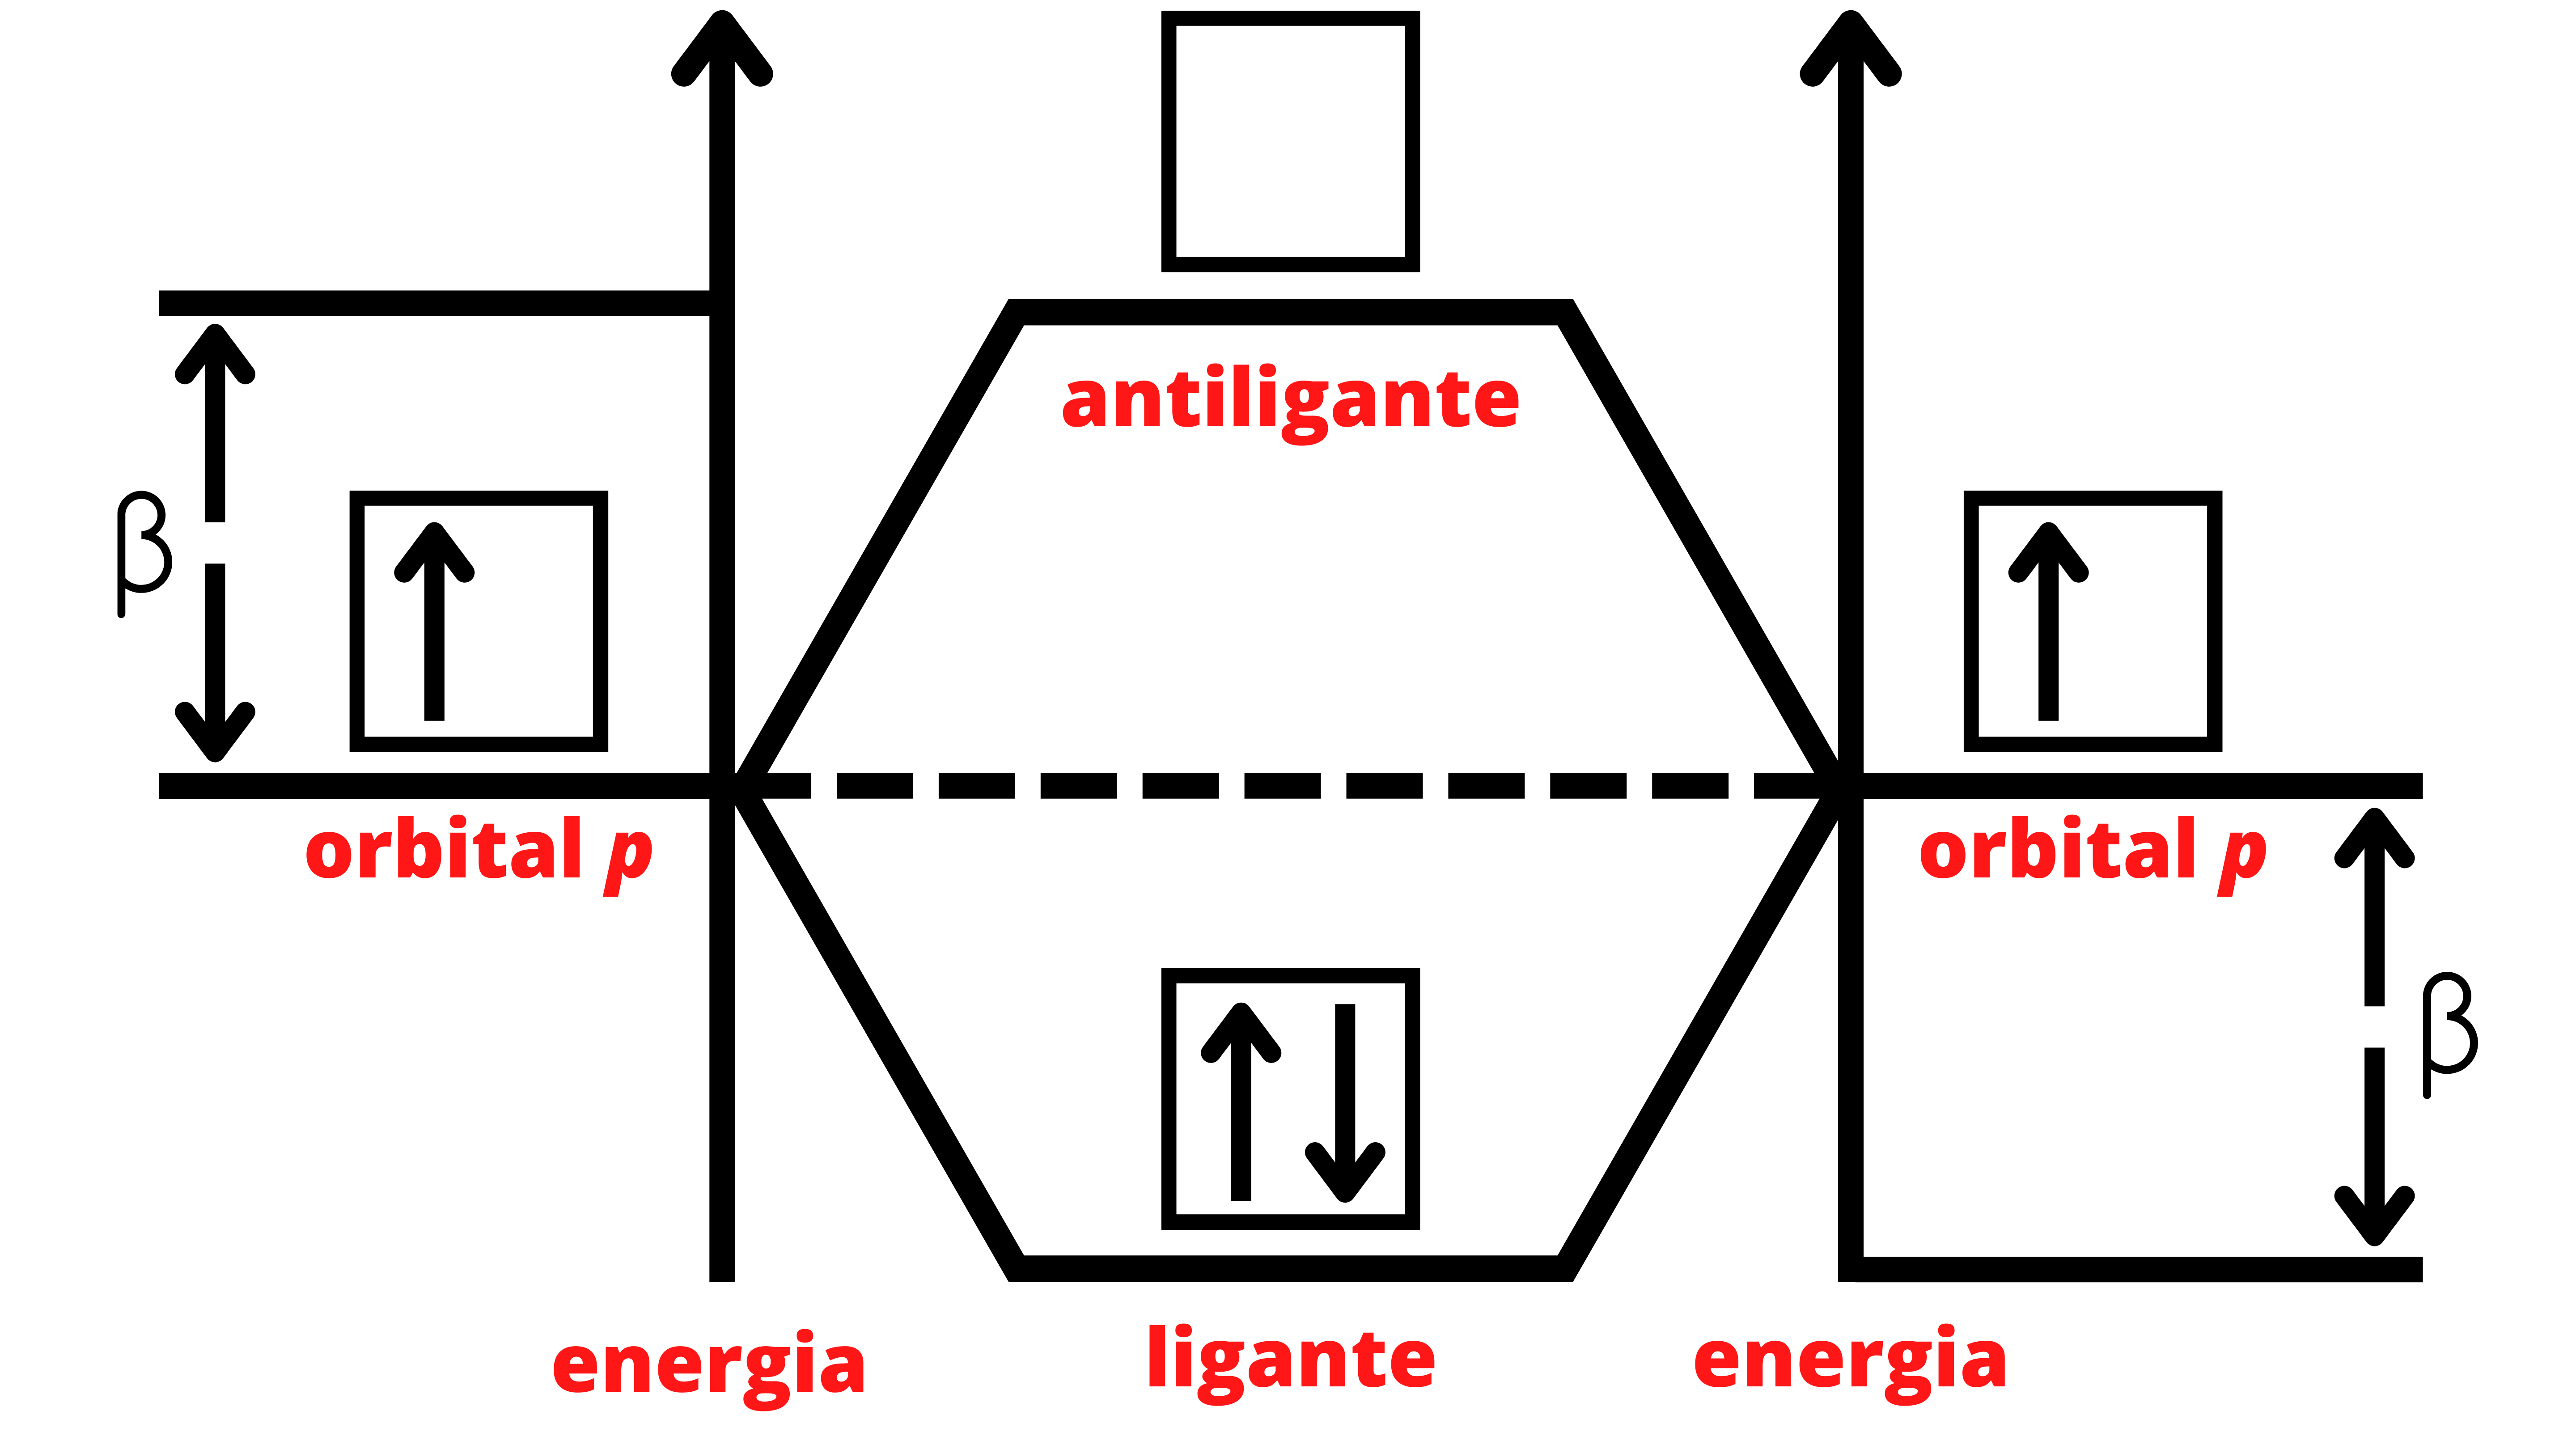
\includegraphics[width=0.75\textwidth]{images/figA2.png}
	\end{center}
	\fonte{Autor(a).}
\end{figure}

Tomemos agora como exemplo um sistema alílico \ce{[CH_2=CH-CH_2-]}, que possui 3 carbonos. Obtém-se, portanto, uma matriz $3 \times 3$ como matriz secular dos coeficientes, cujos elementos seguem as seguintes regras:

\begin{enumerate}
    \item Cada período representa a conectividade do átomo correspondente;
    \item Em cada período, o átomo de referência é rotulado como $x$ (posições $i=j$);
    \item Se $i \neq j$, e se o átomo correspondente é conectado ao respectivo átomo de referência, o elemento de matriz é igual a 1;
    \item Se $i \neq j$, e se o átomo correspondente não é conectado ao respectivo átomo de referência, o elemento de matriz é igual a 0.
\end{enumerate}

\noindent A partir de tais afirmações, a matriz secular será dada pela \autoref{ap:eq:13f}.

\begin{equation}
\label{ap:eq:13f}
\begin{bmatrix}
    x & 1 & 0 \\
    1 & x & 1 \\
    0 & 1 & x 
\end{bmatrix}
\end{equation}

Resolvendo-a por meio do mesmo procedimento empregado anteriormente, obtém-se: $E = \alpha$, $E = \alpha + \beta \sqrt{2}$ e $E = \alpha - \beta \sqrt{2}$, no qual o nível mais baixo de energia será ocupado com dois elétrons obtidos de orbitais não hibridizados dos dois átomos de carbono.

\chapter{Método de Hueckel Estendido} \label{ap:EHMO}

O \gls{EHMO} surgiu como um aprimoramento do procedimento enunciado por Hueckel, considerando todos os elétrons da valência em um cálculo de orbitais moleculares (\autoref{ap:eq:14}). Ou seja, a partir disso, pode-se calcular as barreiras de energia para rotacionar as ligações, e mesmo determinar as energias e estruturas dos estados de transição para reações.

A função de onda eletrônica é considerada, nesse modelo, como um produto de funções de onda monoeletrônicas:

\begin{figure}[htb]
    \vspace{2\baselineskip}
\begin{equation}
    \label{ap:eq:14}
    \psi_{\textbf{total}} = \psi_{\textbf{núcleo}} + \tikzmarknode{hmo}{\highlight{red}{$\psi_{\textbf{valência}}$}}
\end{equation}
\begin{tikzpicture}[overlay,remember picture,>=stealth,nodes={align=left,inner ysep=1pt},<-]
    \path (hmo.north) ++ (1.2em,1.5em) node[anchor=south west,color=red!67] (scalep){\textit{Hueckel estendido}};
    \draw [color=red!87](hmo.north) |- ([xshift=3em,color=red]scalep.south east);
\end{tikzpicture}
\end{figure}

\begin{figure}[htb]
    \vspace{2\baselineskip}
\begin{equation}
    \psi_{\textbf{valência}} = \psi_1 (1) \psi_2 (2) \psi_3 (3) \dots \tikzmarknode{j}{\highlight{red}{$\psi_j$}} (\tikzmarknode{n}{\highlight{blue}{$n$}})
\end{equation}
\begin{tikzpicture}[overlay,remember picture,>=stealth,nodes={align=left,inner ysep=1pt},<-]
    \path (j.north) ++ (1.2em,1.5em) node[anchor=south west,color=red!67] (scalep){$\displaystyle \psi_j = \sum_{r=1}^N c_{jr} \phi_r$};
    \draw [color=red!87](j.north) |- ([xshift=3em,color=red]scalep.south east);
    
    \path (n.south) ++ (1.2em,-1.5em) node[anchor=north west,color=blue!67] (scalep){\textit{$n^o$ de elétrons}};
    \draw [color=blue!87](n.south) |- ([xshift=3em,color=blue]scalep.north east);
\end{tikzpicture}
\end{figure}

\noindent onde $n$ é o número de elétrons e $j$ identifica o orbital molecular. Novamente, cada um dos \gls{MOs} é dada pela LCAO. O conjunto de orbitais aqui definidos são chamados \textit{conjunto mínimo de base}, pois contém somente as informações dos orbitais atômicos para a camada de valência dos átomos. 

\begin{equation}
    HC = SCE
\end{equation}

\noindent onde $H$ é uma matriz quadrada contendo o $H_{rs}$, integrais de energia de um único elétron, e $C$ é a matriz dos coeficientes relativos aos orbitais atômicos. Cada coluna em $C$ é $C'$, que define um orbital molecular em termos das funções de base. Na teoria molecular de Hueckel estendido, a sobreposição não é negligenciado, e $S$ é a matriz das integrais de sobreposição. Essas matrizes são quadradas, possuem o tamanho igual ao número de orbitais atômicos usados na combinação linear. Para qualquer cálculo desse tipo, deve-se construir essas matrizes e então encontrar os autovalores (energias orbitais) e autovetores (coeficientes que definem o orbital molecular em termos das funções de base).

Os elementos da matriz $H$ são atribuídos a partir de dados experimentais, uma vez que o método em questão é semi-empírico. Os elementos de matriz Hamiltoniana fora de diagonal são dados por uma aproximação feita por Wolfsberg e Helmholz, que relaciona com os elementos diagonais e o elemento da matriz de sobreposição, seguindo a \autoref{hamiltonian}. De acordo com essa expressão, a energia deveria ser proporcional à energia dos orbitais atômicos, e será tão maior quanto maior a sobreposição desses orbitais. A contribuição desses efeitos com a energia é escalada pelo fator $K$. Hoffmann \autocite{Hoffmann1963} atribuiu o valor de 1.75 para $K$, após um estudo do efeito desse parâmetro nas energias dos orbitais ocupados do etano.

\begin{figure}[htb]
\label{hamiltonian}
    \vspace{2\baselineskip}
\begin{equation}
    H_{rs} = \frac{1}{2} \tikzmarknode{k}{\highlight{red}{$K$}}(H_{rr} + H_{ss}) \tikzmarknode{s}{\highlight{blue}{$S_{rs}$}}
\end{equation}
\begin{tikzpicture}[overlay,remember picture,>=stealth,nodes={align=left,inner ysep=1pt},<-]
    \path (k.north) ++ (1.2em,1.5em) node[anchor=south west,color=red!67] (scalep){\textit{constante de Wolfsberg-Helmholtz}};
    \draw [color=red!87](k.north) |- ([xshift=3em,color=red]scalep.south east);
    
    \path (s.south) ++ (-1.2em,-1.5em) node[anchor=north east,color=blue!67] (scalep){\textit{integral de sobreposição $\Longrightarrow S_{rs} = \langle \psi_r | \psi_s \rangle$}};
    \draw [color=blue!87](s.south) |- ([xshift=-3em,color=blue]scalep.north west);
\end{tikzpicture}
\end{figure}

A expressão da \autoref{hamiltonian} pode ser racionalizada de forma a tratar a energia dos orbitais atômicos proporcionalmente à energia dos orbitais atômicos, aumentando diretamente de acordo com a integral de sobreposição e sendo escalada peo parâmetro $K$.

 Os valores de $H_{rr}$ (quais sejam, os elementos da diagonal da matriz) são escolhidos como um estado de potenciais de ionização com o valor negativo, indicando ligação. Isso ocorre em função do teorema de Koopman\autocite{Koopmans1934}, cujo enunciado determina que a primeira energia de ionização de um sistema molecular é o oposto da energia atribuída ao \gls{HOMO}, uma vez que. no contexto do \gls{RHF}, considera-se que os orbitais do íon são idênticos àqueles da molécula neutra (segundo a aproximação do orbital \textit{congelado}). 

\begin{table}[htb]
	\centering
	\caption{\label{qua:Quadro_1} Valores de $H_{rr}$ tomados a partir do potencial de ionização.}	
	\begin{tabular}{ccc}
		\toprule
		\textbf{Sítio de ligação} & \textbf{Potencial de ionização/(eV)} & \textbf{Valores de $H_{rr}$/(eV)}
		\\ 
		\midrule
        H-1s & 13.60 & -13.60 \\
        C-2s & 21.40 & -21.40 \\
        C-2p & 11.40 & -11.40 \\
        N-2s & 25.58 & -25.58 \\
        N-2p & 13.90 & -13.90 \\
        O-2s & 32.28 & -32.28 \\
        O-2p & 15.85 & -15.85 \\
        F-2s & 40.20 & -40.20 \\
        F-2p & 18.66 & -18.66 \\
    \bottomrule
	\end{tabular}
	\fonte{\textit{Department of Organic and Polymeric Materials}, \href{t http://www.op.titech.ac.jp/lab/mori/EHTB/EHTB.html}{\textit{Tokyo Institute of Technology}.}}
\end{table}

É comum, em muitos estudos teóricos\autocite{Zubatiuk2021, BroJrgensen2021}, utilizar a metodologia em questão como um passo preliminar para determinar os orbitais moleculares por um método mais sofisticado, mais caro computacionalmente, como cálculo \textit{ab initio}.

\section{Teorema de Koopman}



\chapter{Teoria de grafos} \label{ap:graph}

A Teoria dos Grafos tem uma origem relativamente recente (século XVIII) na
história da Matemática. Desenvolvida já no século XX, cuja importância se tem
imposto por suas ligações e aplicações em outras ciências, bem como em outras
áreas da Matemática, pois estuda as relações entre os objetos de um determinado conjunto\autocite{neto2016topicos, soares2014introduccao}.

Tal conceito simples torna claro que ele permite a modelagem de situações concretas como: redes de computadores, de comunicações, a Web (ligação física entre
os nós da rede), árvores genealógicas, Química Orgânica (isômeros), etc.
Contudo, a ligação física não é necessária; também pode ser associado um grafo
a um qualquer conjunto no qual esteja definida uma relação binária, como a relação
(a é primo com b) que determina um grafo num conjunto fixado de inteiros, ou a
relação (a é filho de b) que permite associar a uma dada família um grafo (árvore
genealógica).


As aplicações químicas da teoria de grafos são altamente úteis, por exemplo, para a enumeração e representação de isômeros constitucionais, como para derivados regioisoméricos de benzeno ou para hidrocarbonetos ramificados. Os cálculos da teoria gráfica envolvem procedimentos combinatórios, para gerar grafos como representações topológicas, e álgebra linear - a formação de matrizes e vetores, a extração de autovalores e  autovetores e operações relacionadas. Todos estes procedimentos são eficiente e rapidamente implementados com programas para computação simbólica\autocite{allinger2010molecular}.

\begin{definition}
Um \textbf{grafo (simples)} G consiste de um conjunto finito e não vazio
V(G) de objetos chamados vértices, juntamente com um conjunto E(G) de pares
não ordenados de vértices; os elementos de E(G) são chamados de \textbf{arestas}. Pode-se representá-lo por G = (V;E), onde V = V(G) e E = E(G).
\end{definition}

Se $G = (V;E)$ é um grafo é um grafo e $u$ e $v$ são dois de seus vértices, diremos que são adjacentes se $\{u,v\} \in E$; neste caso, dizemos ainda que a aresta $\{u,v\}$ incide nos vértices $u$ e $v$. Podemos denotar a aresta simplesmente por $uv$, sempre que não houver risco de confusão. Se $u$ e $v$ não forem adjacentes, diremos que são vértices não adjacentes de $G$.

Grafos são geralmente representados por diagramas, onde os elementos de $V$ correspondem a pontos no plano e as arestas de $G$ correspondem a arcos ligando os vértices correspondentes. A figura assim obtida não tem nenhum significado geométrico, seu propósito sendo somente o de representar esquematicamente as relações de adjacência entre os vértices de $G$ (\autoref{fig:G1}).

\begin{figure}[htb]
	\caption{\label{fig:G1} Imagem representativa de um grafo simples não direcionado.}
	\begin{center}
		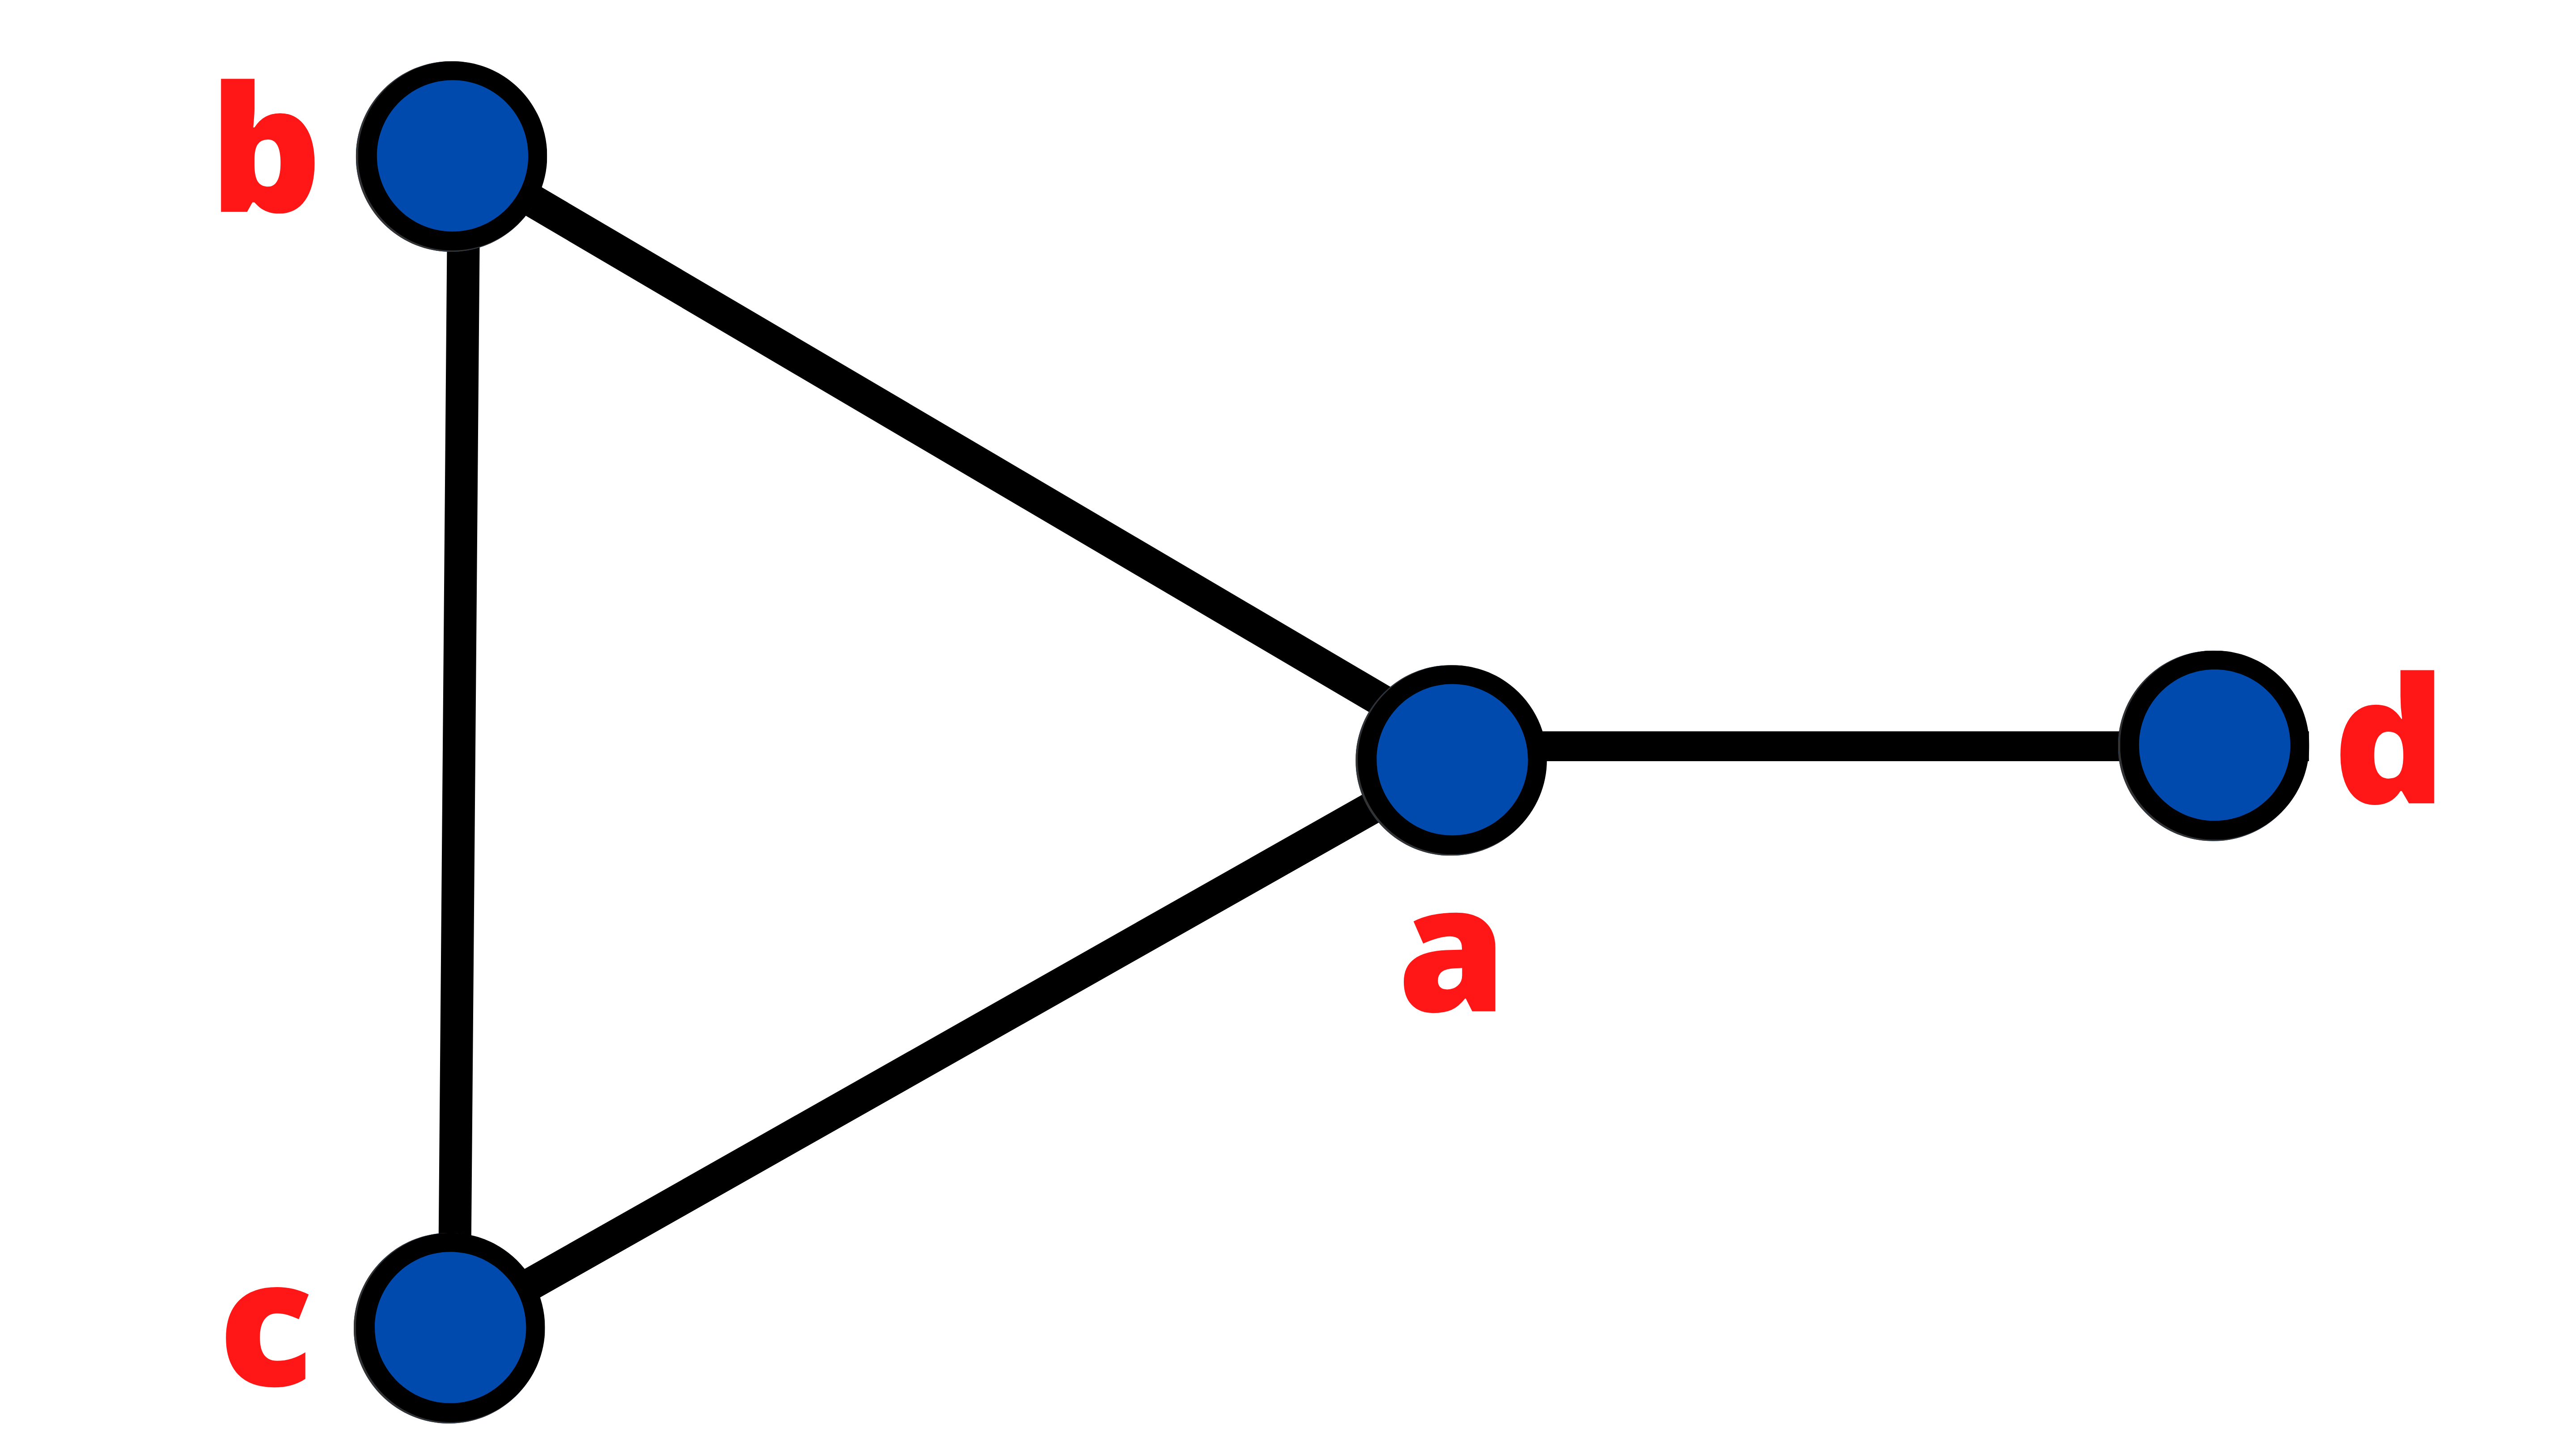
\includegraphics[width=0.6\textwidth]{images/grafo.png}
	\end{center}
	\fonte{Autor(a).}
\end{figure}

\begin{equation}
    G = (\{a,b,c,d\}; \{\{a,b\},\{a,c\},\{a,d\}, \{b,c\}\})
\end{equation}

\begin{definition}
Seja G = (V,E) um grafo. Se u $\in$, o \textbf{grau} de u, denotado $d_G(u)$, é o número de vértices adjacentes a u: 
\begin{center}
$d_G(u) = \#N_G(u)$
\end{center}
\end{definition}

\begin{definition}
Dado um grafo G = (V;E), com |V| = n, suponha que V=$I_n$. A \textbf{matriz de adjacência} de G é a matriz Adj(G) = $(a_{ij})_{n\times n}$, tal que
\begin{center}
\begin{equation*}
a_{ij}= \Bigg{\{} \begin{array}{ll} 1, \; se \; i\neq j  \; e \; \{i,j\} \in E \\ 0, \; se \; \textrm{\textit{não}} \end{array}
\end{equation*}
\end{center}
\end{definition}

De acordo com o grafo da \autoref{fig:G1}, obtemos a matriz de adjacência na \autoref{adj}.

\begin{equation}
\label{adj}
    \begin{bmatrix}
       0 & 1 & 1 & 1 \\
       1 & 0 & 1 & 0 \\
       1 & 1 & 0 & 0 \\
       1 & 0 & 0 & 0 
    \end{bmatrix}
\end{equation}